\section{Auswertung}
\label{sec:Auswertung}
\subsection{Bestimmung des Schubmoduls G}
\begin{equation}
	\theta_{\mathrm{Kugel}}=(1.3197\pm 0.0006) \cdot 10^{-4} \,\si{\kilo\gram \square\metre}
\end{equation}
\begin{equation}
	G= (8.987\pm 0.004) \cdot 10^{10}  \,\si{\newton \per \square\metre}
\end{equation}
\begin{equation}
	Q= (1.056\pm 0.011) \cdot 10^{11}  \,\si{\newton \per \square\metre}
\end{equation}

\begin{equation}
	\mu= 0.1684\pm 0.0028
\end{equation}
%\begin{figure}
%  \centering
%  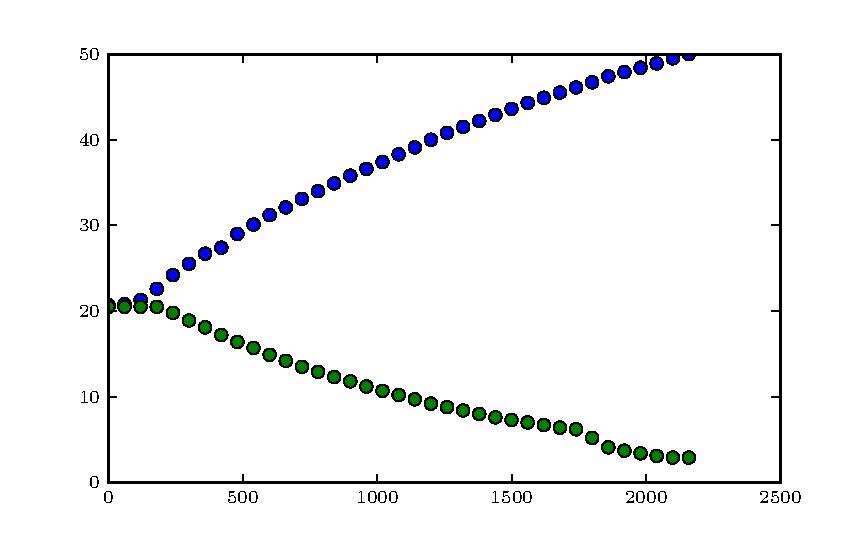
\includegraphics{plot.pdf}
%  \caption{Plot.}
%  \label{fig:plot}
%\end{figure}
E= (2.100+/-0.005)e+11
\subsection{Bestimmung des magnetischen Moments $m$ des Helmholtzspulenpaars}
Das B-Feld eines Helmholtzspulenpaars ergibt sich mit
\begin{equation}
	B_{\mathrm{H}}=
\end{equation}



a = m = 0.0338563481372 +- 0.000438666200483
b = D =  7.434181548e-06 +- 1.22371249137e-06


%%%%%%%%%%%%%%%%%%%%%%%%%%%%%%%%%%%%%%%%%%%%%%%%%%%%%%%%%%%%%%%%%%%%%%%%%%%%%%%%%%%%%%%%%%%
\FloatBarrier
\subsection{Bestimmung der Horizontalkomponente des Erdmagnetfeldes}

Die Messwerte der Periodendauer $T$ der Drehschwingung zur Bestimmung der Horizontalkomponente 
des Erdmagnetfeldes sind in Tabelle \ref{tab:magnetusmaximus} aufgetragen.
\begin{table}
	\caption{Messwerte der Periodendauer $T$ zur Bestimmung der Horizontalkomponente 
	des Magnetfeldes.}
	\label{tab:magnetusmaximus}
	\centering
	\begin{tabular}{cc}
		\toprule
		Nummer & $T$/$\si{\second}$ \\
		\midrule
		1 & 19.957 \\
		2 & 19.948 \\
		3 & 19.949 \\
		4 & 19.940 \\
		5 & 19.944 \\
		6 & 19.944 \\
		7 & 19.936 \\
		8 & 19.933 \\
		9 & 19.937 \\
		10 & 19.930 \\
		\bottomrule
	\end{tabular}
\end{table}
Damit ergibt sich die Periodendauer $T$ als Mittelwert (bestimmt mit Formel
\eqref{eqn:mittelwert} dieser Messwerte mit zugehörigem Fehler (bestimmt mit Formel
\eqref{eqn:mittelwertfehler}) zu 
\begin{equation*}
	T = (19,942 \pm 0,003) \, \si{\second} \mathrm{.}
\end{equation*}

Die Horizontalkomponente des Erdmagnetfeldes ergibt sich durch Formel \eqref{eqn:periodemagnet} 
und der Richtgröße eines Zylinders $D$ (Formel \eqref{eqn:richti}) zu
\begin{equation}
	B = 4\pi^2\frac{\theta}{m T^2} - \frac{\pi G R^4}{2Lm} \mathrm{.} 
\end{equation}
